% t = top align slides, alternative c = center
% handout/final = bullet points etc. one by one (final) or all on the slide immediately (handout)
\documentclass[t,xcolor={dvipsnames},final,aspectratio=169]{beamer}
\beamertemplatenavigationsymbolsempty
\usepackage{adjustbox}

\mode<presentation> {
	\usetheme{Frankfurt}
	\usecolortheme{crane}
	\setbeamertemplate{footline}[frame number]
	\beamerdefaultoverlayspecification{<+->}
}

\title{Unit 5.2:
Large Language Models}

\author{Utrecht Summer School: 
Programming with Python 2025}
\institute[UU]{
%All icons by: https://www.flaticon.com/
}
\date{2025-07-11}
\logo{
\includegraphics[scale=0.5]{UU-logo2011_CMYK}\hspace*{0.65\textwidth}\vspace{-8mm}}
\begin{document}
\begin{frame}
\maketitle
\end{frame}

{\setbeamertemplate{logo}{}
\begin{frame}
\frametitle{Table of Contents}
\tableofcontents
\end{frame}
}

\section{What is an LLM}
\begin{frame}{Stupid is as stupid does}
\begin{itemize}
\item What do you think is the next word that I will...?
\end{itemize}
\end{frame}
\begin{frame}{Stupid is as stupid does}
\begin{itemize}
\item What do you think is the next word that I will WRITE?
\item What do you think is the next word that I will SAY?
\item How did you guess?
\end{itemize}
\end{frame}

\begin{frame}{LLMs as coding agents}
\texttt{a = [2, 4, 5]}
\pause

\texttt{\# Compute the mean of the list}
\pause

Can the LLM auto-complete?
\end{frame}

{\setbeamertemplate{logo}{}
\begin{frame}{LLMs as bug fixers}
\texttt{\# Create a dictionary with elements in the name of a person}
\texttt{name\_parts = \{"given name": "Consolacion", "surname": "Valenzuela"\}} \\
\texttt{\# Add a middle name}\\
\texttt{name\_parts.append("middle name": "Celestina")}

\pause
\vfill
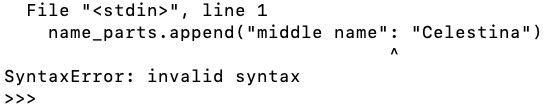
\includegraphics[width=8cm]{error.png}

\pause
\vfill
\includegraphics<+->[width=8cm]{llm.png}
\end{frame}
}

\section{Ethics}
\begin{frame}{Training data}
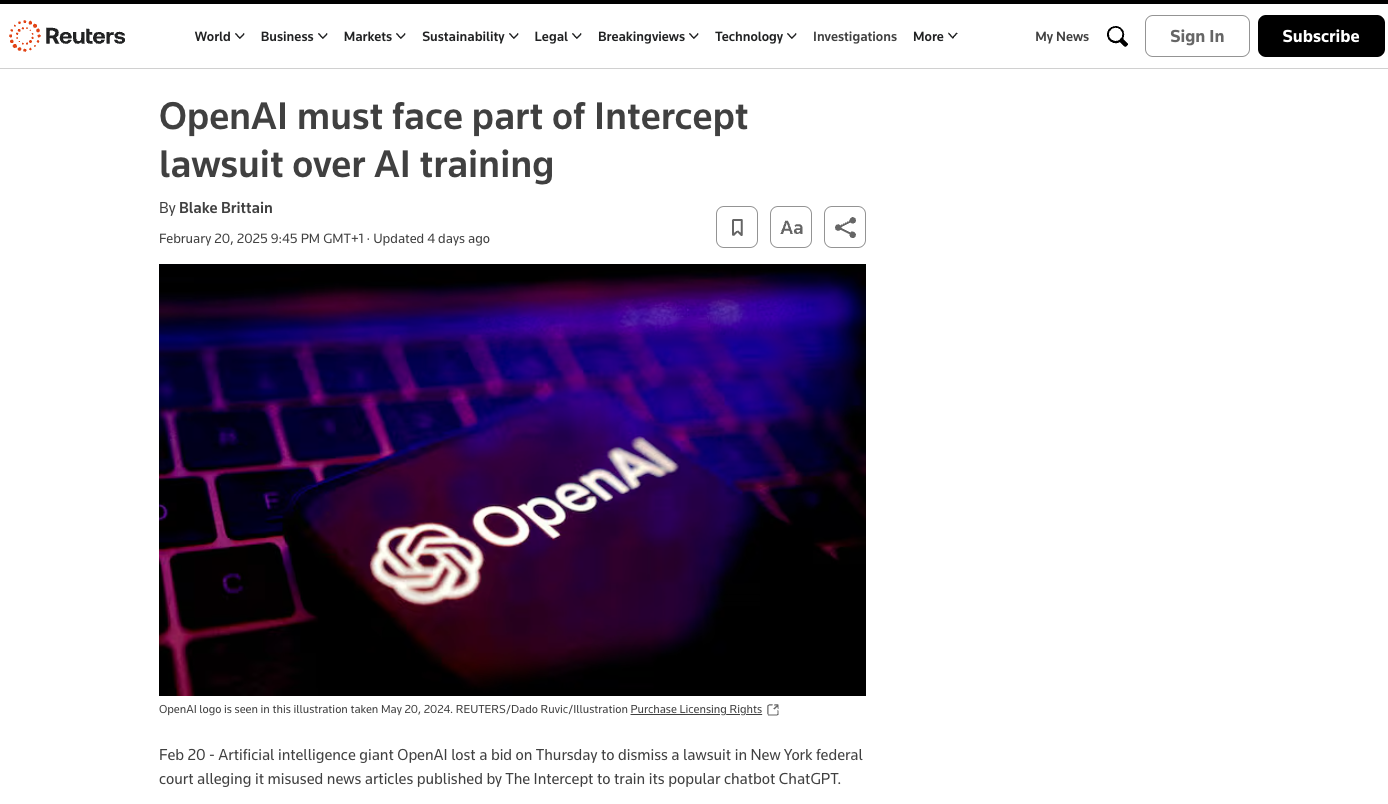
\includegraphics[width=\textwidth]{trainingdata.png}
\end{frame}

{\setbeamertemplate{logo}{}
\begin{frame}{Environment}
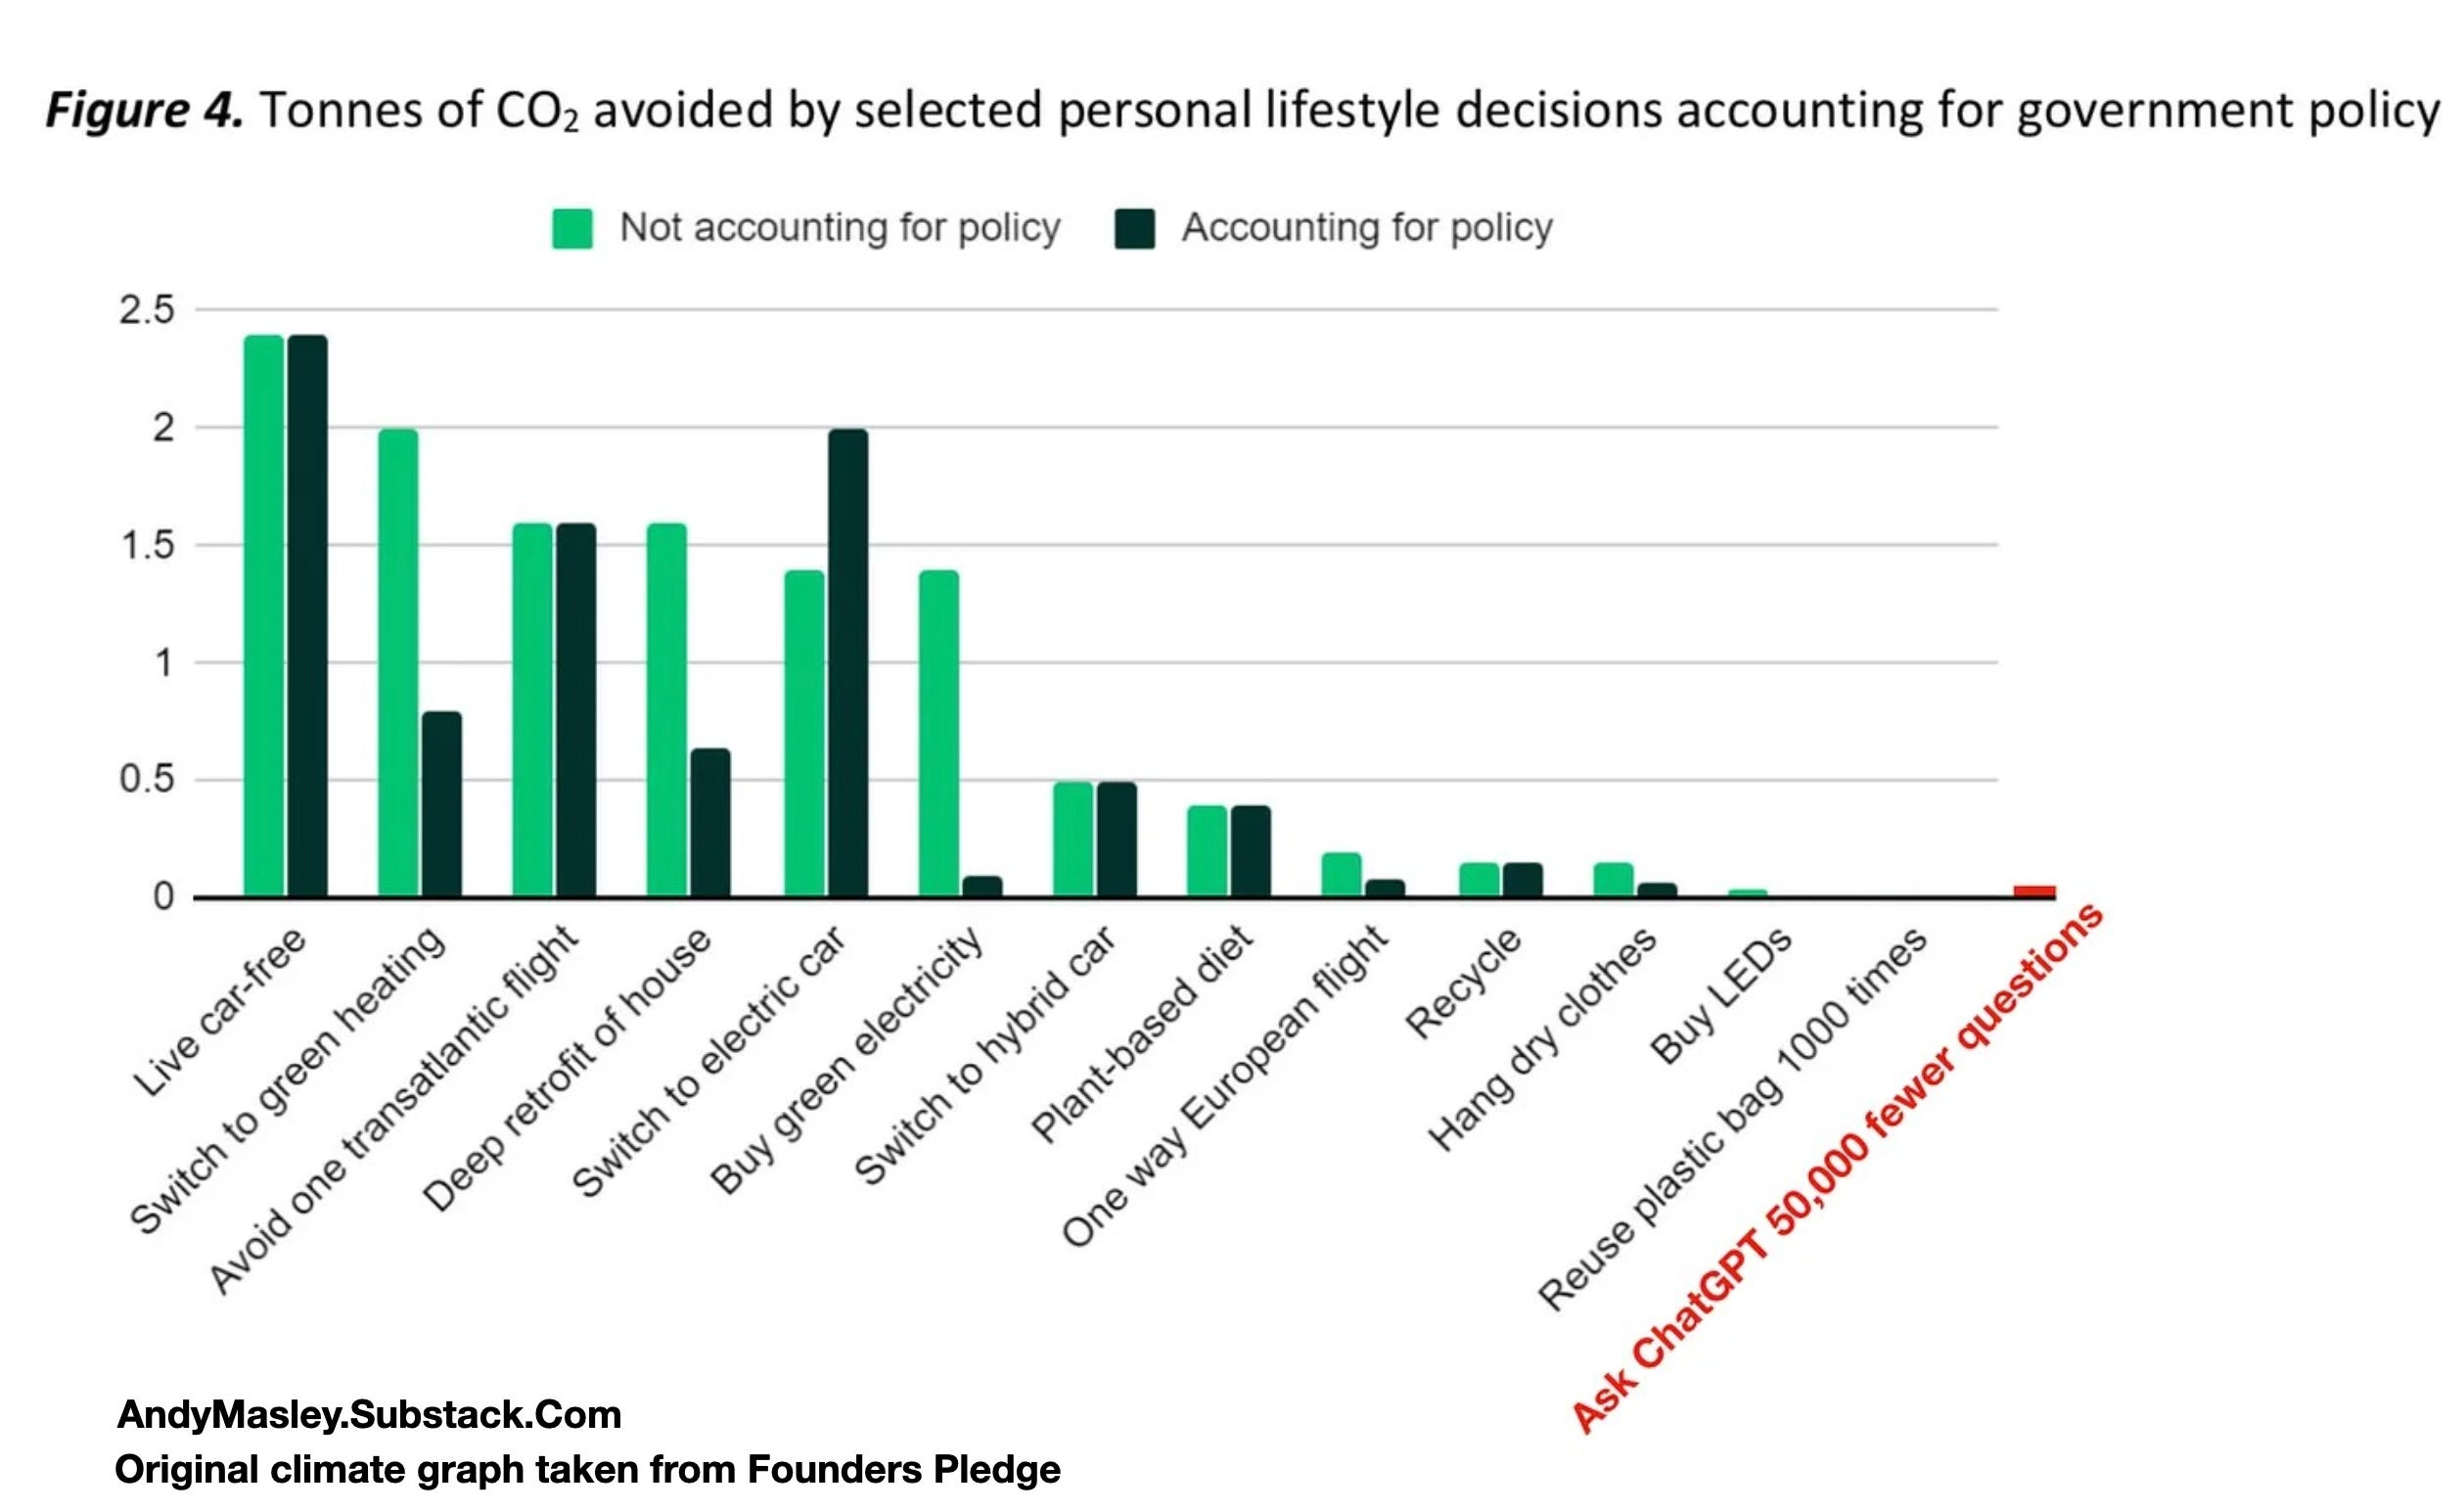
\includegraphics[width=0.7\textwidth]{emissions.jpg}
\footnote{Source (January 2025): \url{https://open.substack.com/pub/andymasley/p/individual-ai-use-is-not-bad-for}}
\end{frame}
}

{\setbeamertemplate{logo}{}
\begin{frame}{Labor conditions}
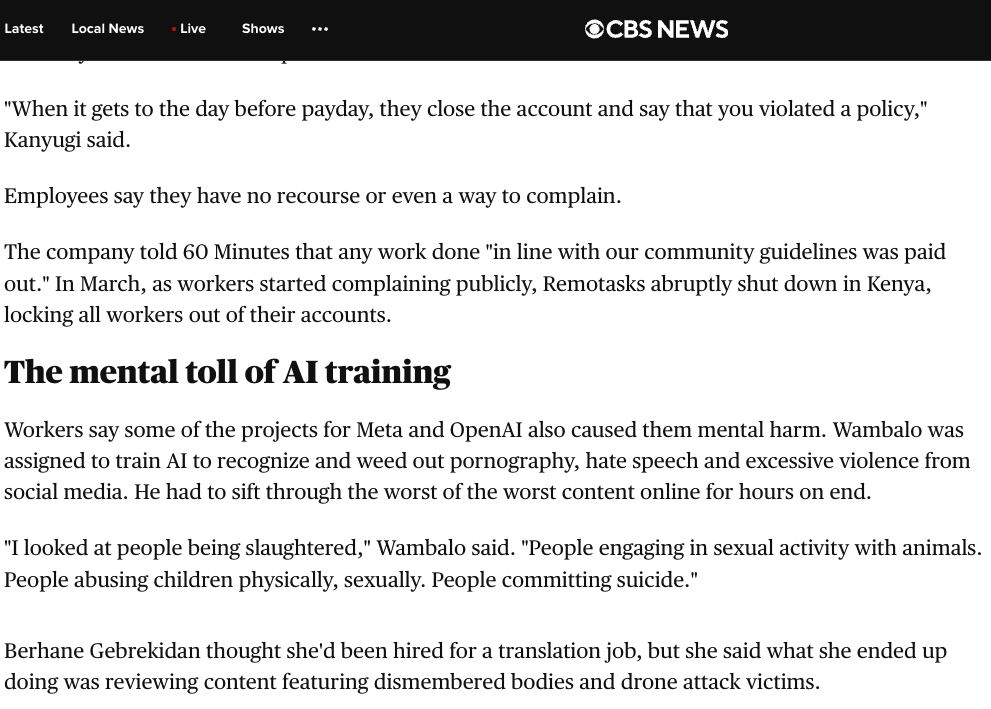
\includegraphics[width=0.6\textwidth]{labor.png}
\footnote{Source (November 2024): \url{https://www.cbsnews.com/news/ai-work-kenya-exploitation-60-minutes/}}
\end{frame}
}

{\setbeamertemplate{logo}{}
\begin{frame}{Effect on cognition}
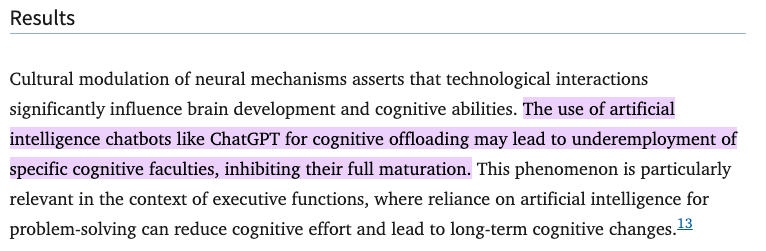
\includegraphics[width=0.6\textwidth]{cognition.png}
\footnote{Source (June 2024): Dubey et al. Redefining Cognitive Domains in the Era of ChatGPT: A Comprehensive Analysis of Artificial Intelligence's Influence and Future Implications. Med Res Arch. 2024 Jun;12(6):5383. doi: 10.18103/mra.v12i6.5383}
\end{frame}
}

\begin{frame}{Uploading restricted data}
\includegraphics<+->[width=8cm]{llm.png}
\begin{itemize}
\item What if error contains sensitive information?
\end{itemize}
\includegraphics<+->[width=8cm]{municipalitiescode.png}
\includegraphics<+->[width=8cm]{municipalitieserror.png}
\end{frame}

\begin{frame}{Uploading restricted data}
\includegraphics<+->[width=8cm]{municipalitiescode.png}
\includegraphics<+->[width=8cm]{municipalitieserror.png}
\includegraphics<+->[width=8cm]{llm.png}
\begin{itemize}
\item Corrected code is useless / does not work
\end{itemize}
\end{frame}

\begin{frame}{Uploading restricted data}
\includegraphics<+->[width=8cm]{llmdata.png}
\begin{itemize}
\item May be illegal!
\end{itemize}
\end{frame}

\section{HuggingChat}

{\setbeamertemplate{logo}{}
\begin{frame}{HuggingChat}
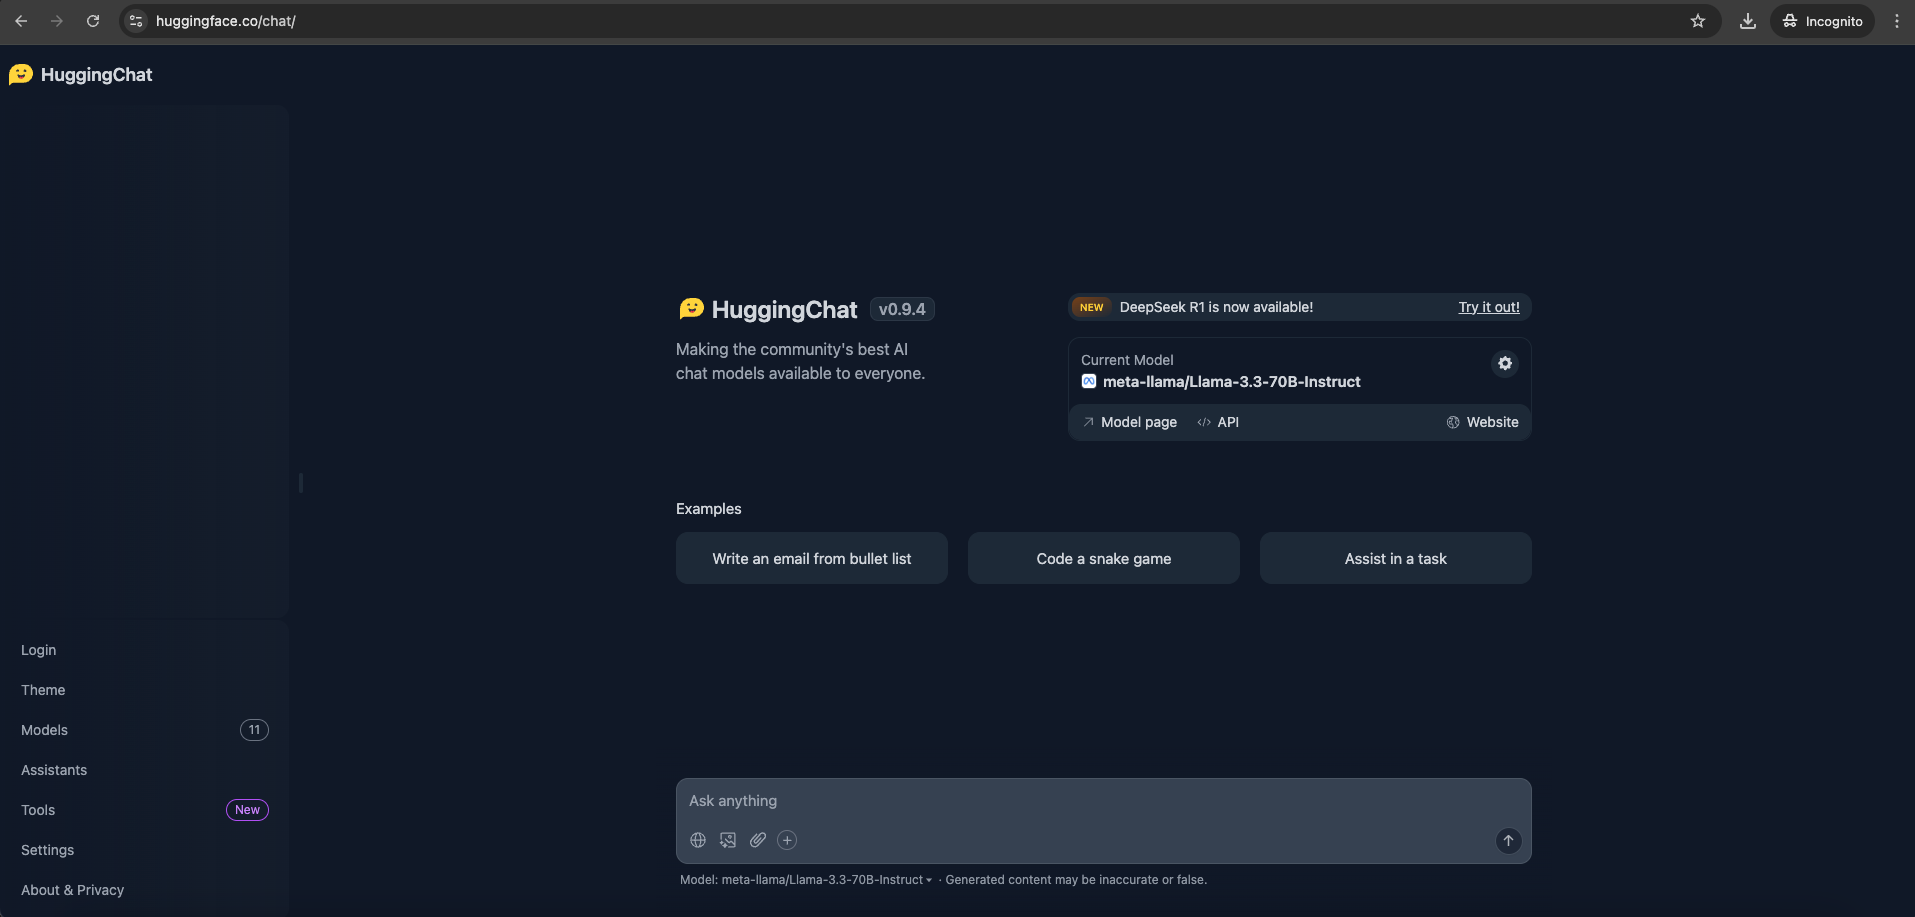
\includegraphics[width=0.9\textwidth]{huggingchat.png}
\end{frame}
}

\begin{frame}{Switch models}
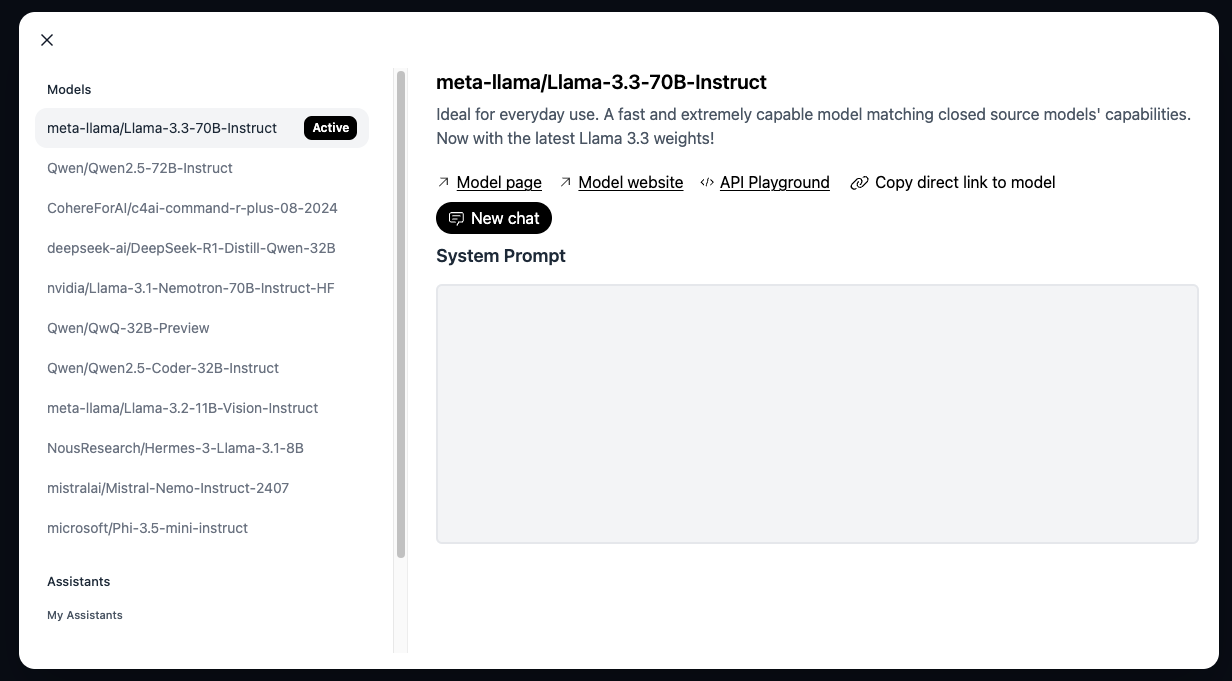
\includegraphics[width=0.9\textwidth]{models.png}
\end{frame}

\section{Colab}
{\setbeamertemplate{logo}{}
\begin{frame}{Generative AI on Google Colab}
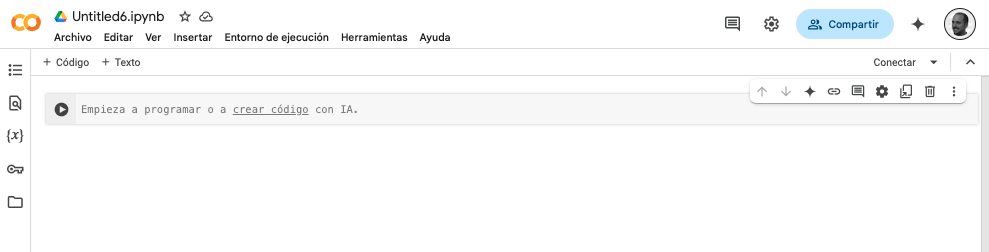
\includegraphics[width=0.8\textwidth]{colab.png}
\pause
\vfill

\includegraphics[width=0.5\textwidth]{gemini.png}
\end{frame}
}

\begin{frame}{Model cards}
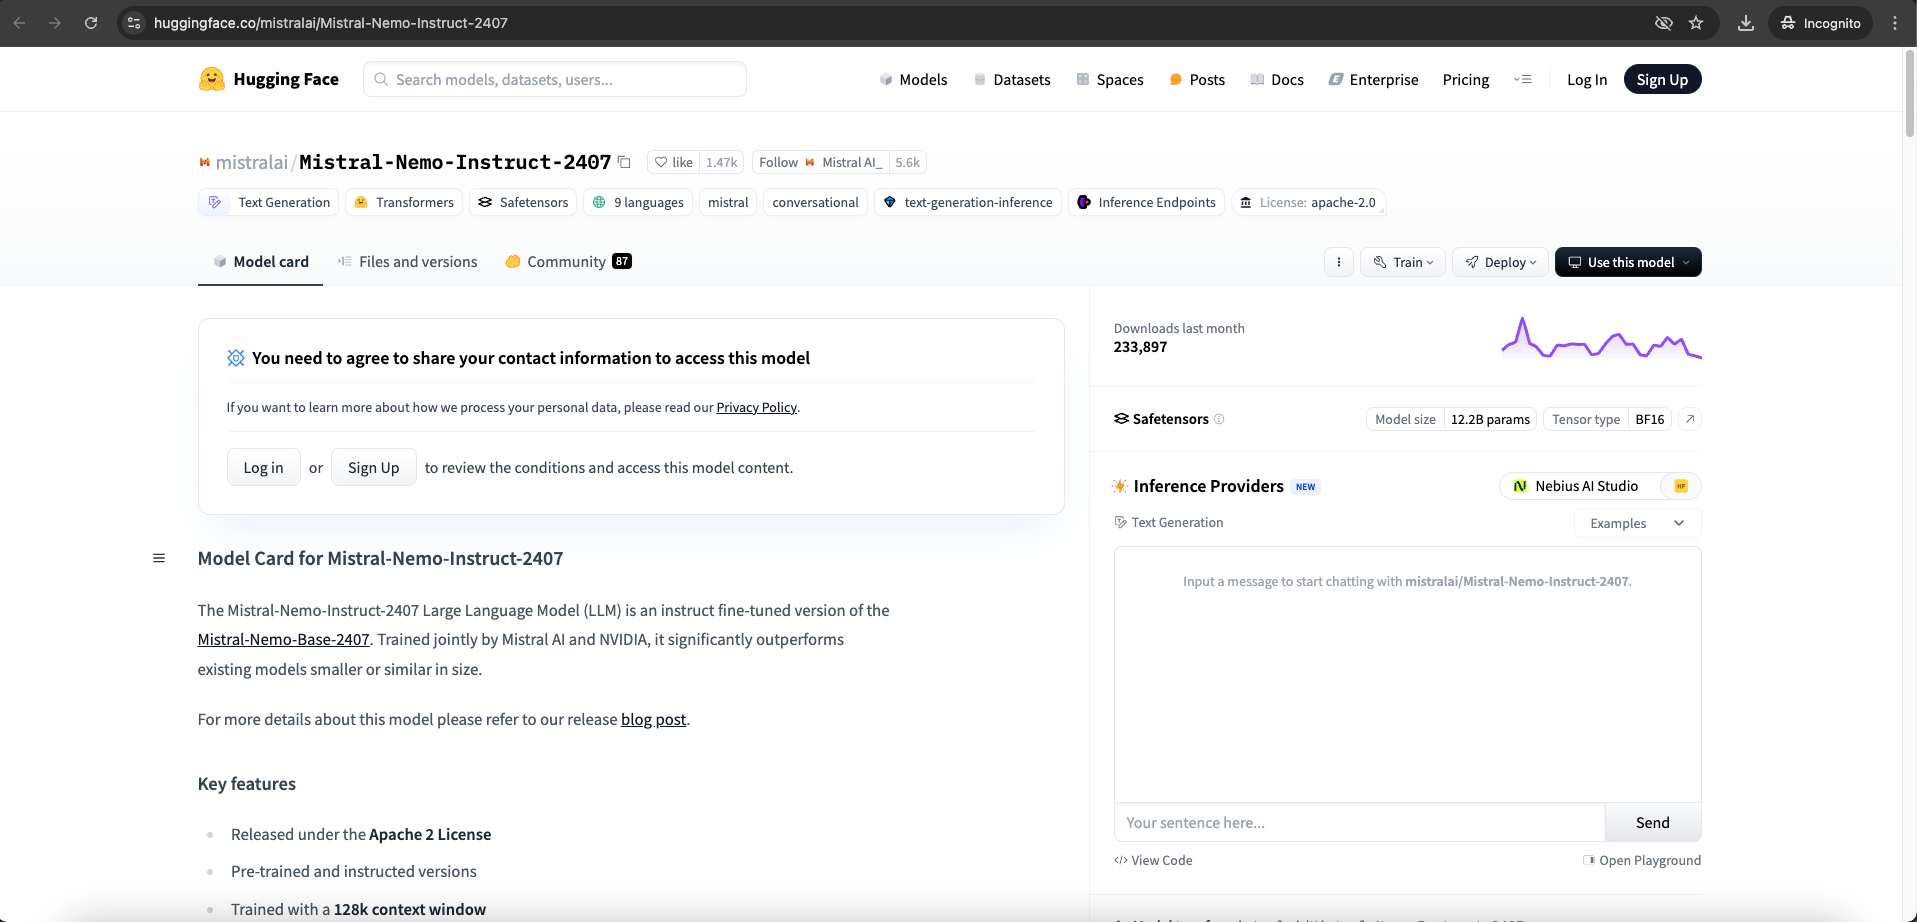
\includegraphics[width=0.7\textwidth]{modelcard.png}
\pause

No model card for Gemini!
\end{frame}

\section{Local LLMs}

{\setbeamertemplate{logo}{}
\begin{frame}{Using an LLM locally (no server)}
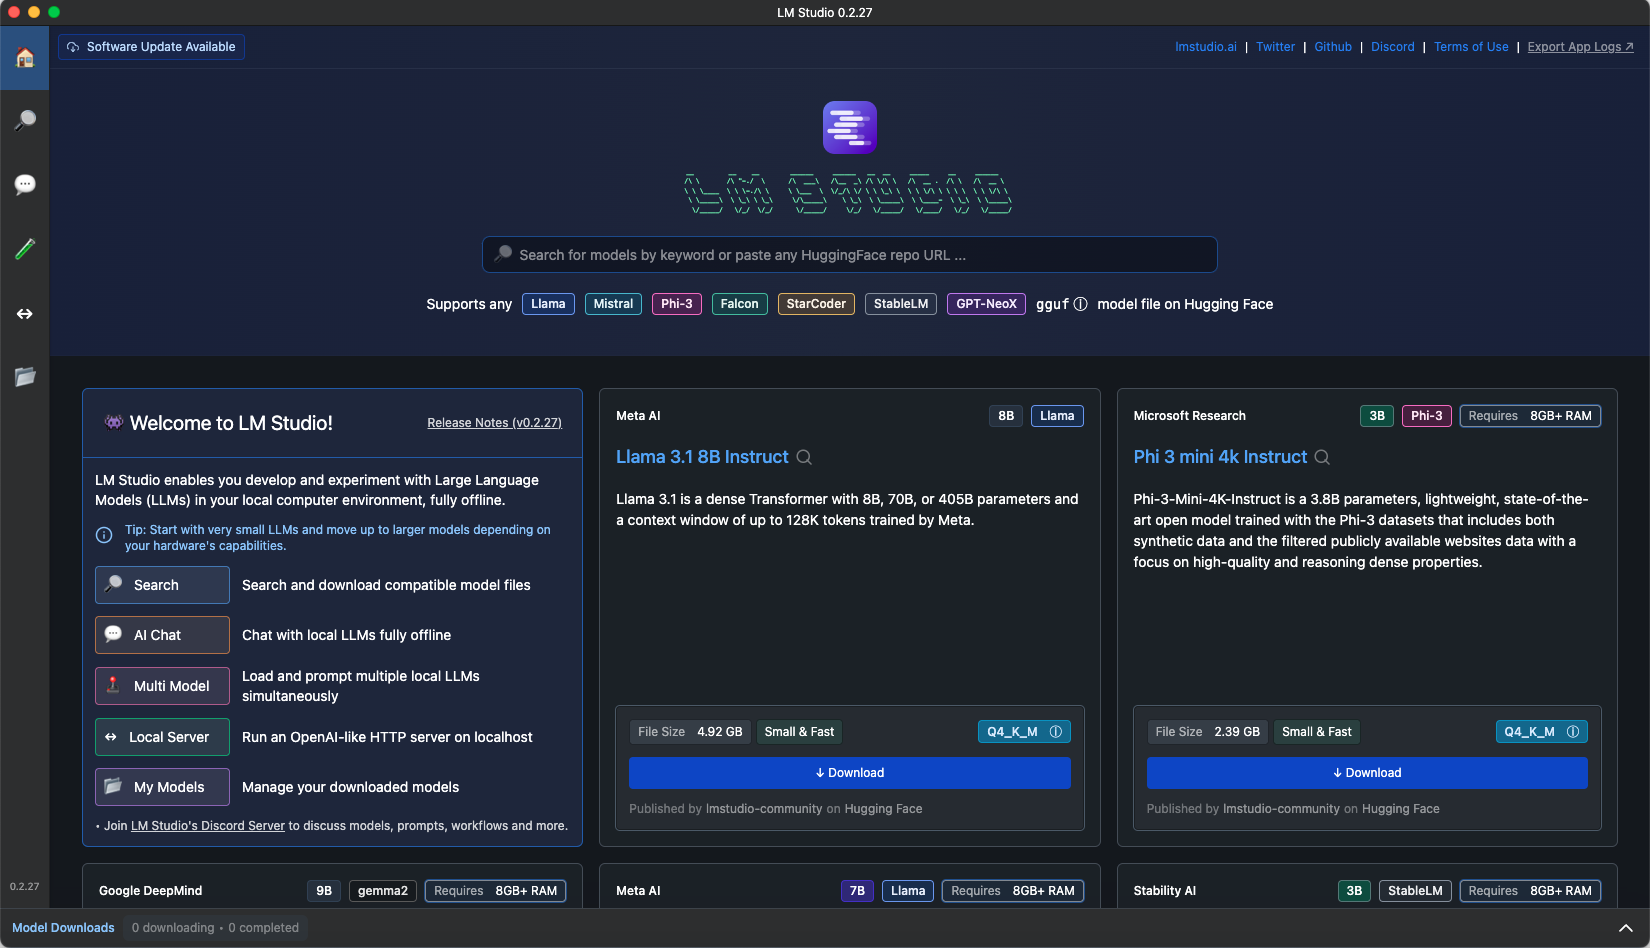
\includegraphics[width=0.8\textwidth]{lmstudio.png}
\end{frame}
}

\section{Conclusions}
\begin{frame}{Time for a demo}
But before we do that...
\begin{itemize}
\item Choose your poison carefully / Know what you choose
\item Do not share private data
\item Consider if you really need this
\end{itemize}
\end{frame}

\end{document}
